\chapter[EXPERIMENTOS, RESULTADOS E DISCUSSÃO]{EXPERIMENTOS, RESULTADOS E DISCUSSÃO}

Neste capítulo serão apresentados e discutidos os resultados obtidos através do processamento dos áudios descritos no capítulo anterior. O principal objetivo é mapear como foi o acerto das ferramentas de transcrição usadas nos experimentos: Google Speech API e Wit.ai. Primeiro serão apresentadas as métricas de forma geral, depois por sotaque regional, por gênero e por grau de escolaridade.

\section{TRATAMENTO DA BASE DE DADOS BRACCENT}

É importante compreender que o trabalho da  \citeonline{batista2019estudo} teve como objetivo a identificação do sotaque regional e que este trabalho versa sobre a transcrição da fala. Assim, no trabalho de origem, não houve a verificação se cada palavra da frase era pronunciado corretamente pelo voluntário. Para este trabalho, foi feita a seguinte verificação, para cada áudio foram ouvidos pelos menos as duas primeiras palavras. Com isso, alguns áudios foram descartados, pois a pessoa não estava falando a frase identificada e haviam repetições de frases pela mesma pessoa, o  \autoref{Tabela_resumo_sotaque} tem a quantidade de áudio por sotaque e por sexo que foi usada. 


% Please add the following required packages to your document preamble:
% \usepackage{multirow}
\begin{quadro}[h]
\caption{Base de dados selecionada para os experimentos por sotaque e por sexo, totalizando 1.648 áudios, 854 femininos e 794 masculinos.} \label{Tabela_resumo_sotaque}
\centering
\begin{tabular}{|c|c|c|c|}
\hline
\textbf{Sotaque}            & \textbf{Sexo} & \textbf{Quantidade de áudio} & \textbf{Total}       \\ \hline
\multirow{2}{*}{Baiano}   & Feminino      & 99                            & \multirow{2}{*}{173}  \\ \cline{2-3}
                            & Masculino     & 74                           &                     \\ \hline
\multirow{2}{*}{Carioca}     & Feminino      & 47                          & \multirow{2}{*}{81} \\ \cline{2-3}
                            & Masculino     & 34                           &                      \\ \hline
\multirow{2}{*}{Fluminense}    & Feminino      & 61                           & \multirow{2}{*}{110} \\ \cline{2-3}
                            & Masculino     & 49                           &                      \\ \hline
\multirow{2}{*}{Mineiro}    & Feminino      & 58                           & \multirow{2}{*}{137}  \\ \cline{2-3}
                            & Masculino     & 79                           &                      \\ \hline
\multirow{2}{*}{Nordestino} & Feminino      & 158                           & \multirow{2}{*}{333} \\ \cline{2-3}
                            & Masculino     & 175                           &                      \\ \hline
\multirow{2}{*}{Nortista} & Feminino      & 6                          & \multirow{2}{*}{24} \\ \cline{2-3}
                            & Masculino     & 18                          &                      \\ \hline
\multirow{2}{*}{Sulista}    & Feminino      & 425                          & \multirow{2}{*}{790} \\ \cline{2-3}
                            & Masculino     & 365                          &                      \\ \hline
\end{tabular}
\fonte{elaborado pelo próprio autor (2021) com os dados do Braccent.}
\end{quadro}


O trabalho original usava 1.743 amostras de fala, enquanto este trabalho usa 1.648 áudios, sendo 95 áudios a menos. Em comparação com as informações do trabalho original, há 10 áudios a menos no Baiano (4 a menos no feminino e 6 a menos no masculino); 1 a menos no Carioca para o gênero masculino; 4 a menos no fluminense (2 a menos em cada gênero); 11 áudios a menos no sotaque mineiro (5 a menos no feminino e 6 a menos no masculino); 11 a menos no Nordestino (sendo 16 a menos no masculino, mas 5 a mais no feminino); 3 a menos no Nortista (2 a menos no feminino e 1 a menos no masculino) e; 55 a menos no sulista (10 a menos no feminino e 45 a menos no masculino). Os áudios foram conferidos e não se encontrou explicação do porque terem mais áudios do sotaque nordestino feminino na base utilizada. 


\begin{quadro}[h!]
\caption{Base de dados selecionada para os experimentos filtrada por grau de ensino, totalizando 1.648 áudios}
\label{Tabela_resumo_grauDeEnsino}
\centering
\begin{tabular}{|l|c|}
\hline
\textbf{Grau de Ensino} & \multicolumn{1}{l|}{\textbf{Quantidade de áudio}} \\ \hline
Médio Incompleto        & 36                                                \\ \hline
Médio Completo          & 109                                               \\ \hline
Superior Incompleto     & 391                                               \\ \hline
Superior Completo       & 712                                               \\ \hline
Mestrado                & 243                                               \\ \hline
Doutorado               & 157                                               \\ \hline
\end{tabular}
\fonte{elaborado pelo próprio autor (2021) com os dados do Braccent.}
\end{quadro}



O \autoref{Tabela_resumo_grauDeEnsino} apresenta a quantidade de áudios por grau de ensino e por sotaque. Mais detalhes encontram-se no Apêndice A, com dados de grau de escolaridade e município/UF de cidade e estado onde o voluntário reside ou de onde o voluntário considera ser o seu sotaque. Logo, a informação de cidade não é muito confiável, dado que o preenchimento foi feito pelo próprio voluntário e a cidade onde reside não define o seu sotaque, e ainda o voluntário pode considerar que tem um determinado sotaque, mas pode estar enganado. O trabalho original contou com a participação de alunos do curso de Letras da Unicamp para fazer a classificação manual.


Nas próximas seções apresentam os resultados e discussão de forma geral, posteriormente separados por sotaque regional, por gênero e por grau de escolaridade. Em cada seção são apresentados os resultados considerando a pontuação das frases: vírgulas, pontos finais, aspas e parágrafos; e sem considerar a pontuação. 

\section{RESULTADO GERAL}

Nesta seção, consideramos os resultados de toda a base de dados testada. O \autoref{Tabela_geral_com_pontuacao} apresenta os resultados do Google Cloud e do Wit.ai considerando a pontuação e o  \autoref{Tabela_geral_sem_pontuacao} sem a pontuação, os melhores resultados estão em negrito para facilitar a comparação, sendo contabilizado um acerto cada transcrição que fosse igual a frase original.

%COM PONTUAÇÃO
\begin{quadro}[h]
\caption{Resultado das APIs considerando a pontuação} \label{Tabela_geral_com_pontuacao}
\centering
\begin{tabular}{c|c|r|r|l}
\cline{1-4}
\multicolumn{1}{|c|}{Métrica}                                 & Estatística  & \multicolumn{1}{c|}{Google Cloud} & \multicolumn{1}{c|}{Wit.ai} &  \\ \cline{1-4}
\multicolumn{1}{|c|}{\multirow{2}{*}{Levenshtein}}            & Média        & 18,29                           & \textbf{5,85}                      &  \\ \cline{2-4}
\multicolumn{1}{|c|}{}                                        & Mediana      & 14                                & \textbf{4}                           &  \\ \cline{1-4}
\multicolumn{1}{|c|}{\multirow{2}{*}{Normalized Levenshtein}} & Média        & 89\%                            & \textbf{96\%}                      &  \\ \cline{2-4}
\multicolumn{1}{|c|}{}                                        & Mediana      & 91\%                            & \textbf{97\%}                  &  \\ \cline{1-4}
\multicolumn{1}{l|}{}                                         & \# Acertos   & 0                                 & \textbf{81}                          &  \\ \cline{2-4}
\multicolumn{1}{l|}{}                                         & \% de Acerto & 0                                 & \textbf{4,91\%}               &  \\ \cline{2-4}
\end{tabular}
\fonte{elaborado pelo próprio autor (2021)}
\end{quadro}


%SEM PONTUAÇÃO
\begin{quadro}[h]
\caption{Resultado das APIs sem considerar a pontuação} \label{Tabela_geral_sem_pontuacao}
\centering
\begin{tabular}{c|c|r|r|l}
\cline{1-4}
\multicolumn{1}{|c|}{Métrica}                                 & Estatística  & \multicolumn{1}{c|}{Google Cloud} & \multicolumn{1}{c|}{Wit.ai} &  \\ \cline{1-4}
\multicolumn{1}{|c|}{\multirow{2}{*}{Levenshtein}}            & Média        & 13,54                           & \textbf{3,21}                      &  \\ \cline{2-4}
\multicolumn{1}{|c|}{}                                        & Mediana      & 9                                 & \textbf{2}                           &  \\ \cline{1-4}
\multicolumn{1}{|c|}{\multirow{2}{*}{Normalized Levenshtein}} & Média        & 92\%                            & \textbf{98\%}                      &  \\ \cline{2-4}
\multicolumn{1}{|c|}{}                                        & Mediana      & 94\%                            & \textbf{98\%}                      &  \\ \cline{1-4}
\multicolumn{1}{l|}{}                                         & \# Acertos   & 126                               & \textbf{543}                         &  \\ \cline{2-4}
\multicolumn{1}{l|}{}                                         & \% de Acerto & 7,64\%                            & \textbf{32,94\%}             &  \\ \cline{2-4}
\end{tabular}
\fonte{elaborado pelo próprio autor (2021)}
\end{quadro}

Acertar a pontuação é um desafio, logo os resultados considerando a pontuação são piores que sem considerá-la. Mesmo assim, o Wit.ai acertou 81 áudios completos com pontuação. O Google Cloud não retorna resultado com pontuação, logo, a indicação de 0 (zero) acertos.  Ressalta-se que sem considerar a pontuação, essa quantidade aumenta em 6,7 vezes, acertando 543 áudios. Em ambos os quadros, é possível verificar que o Wit.ai teve resultados melhores, em todas as estatísticas, que o Google Cloud. 

\FloatBarrier

\section{RESULTADO POR SOTAQUE REGIONAL}

Nesta seção serão discutidos os resultados por sotaque. O \autoref{Tabela_sotaque_Google_com_pontuacao} apresenta os resultados do Google Cloud considerando a pontuação para os diferentes sotaques e o \autoref{Tabela_sotaque_Google_sem_pontuacao} são os resultados sem considerar a pontuação. Para esta ferramenta, é interessante observar que obteve melhores resultados para o sotaque baiano seguido do nordestino. E que em termos do Levenshtein Normalizado, o pior resultado foi para o sotaque carioca e que não houve um único acerto para o sotaque nortista. 


%SEM PONTUAÇÃO
\begin{quadro}[h]
\caption{Resultado do Google Cloud considerando a  pontuação para os diferentes sotaques (Flu = Fluminense, Norde = Nordestino, Nort = Nortista, Sul = Sulista)} \label{Tabela_sotaque_Google_com_pontuacao}
\begin{tabular}{c|l|r|r|r|r|r|r|r|}
\hline
\multicolumn{1}{|c|}{Google Cloud}                                                                       & Estatísticas   & \multicolumn{1}{l|}{Baiano} & \multicolumn{1}{l|}{Carioca} & \multicolumn{1}{l|}{Flu} & \multicolumn{1}{l|}{Mineiro} & \multicolumn{1}{l|}{Norde} & \multicolumn{1}{l|}{Nort} & \multicolumn{1}{l|}{Sul} \\ \hline
\multicolumn{1}{|c|}{\multirow{2}{*}{Levenshtein}}                                                       & Média         & \textbf{13,84}              & 42,17                       & 18,22                      & 22,26                        & 15,62                      & 18,20                         & 17,25                        \\ \cline{2-9} 
\multicolumn{1}{|c|}{}                                                                                   & Mediana       & 13                          & 28                           & 14                         & 14                           & \textbf{12}                         & 14,5                          & 14                           \\ \hline
\multicolumn{1}{|c|}{\multirow{2}{*}{\begin{tabular}[c]{@{}c@{}}Normalized \\ Levenshtein\end{tabular}}} & Média         & \textbf{0,92}                        & 0,75                         & 0,89                       & 0,87                         & 0,91                       & 0,89                          & 0,90                         \\ \cline{2-9} 
\multicolumn{1}{|c|}{}                                                                                   & Mediana       & \textbf{0,92}                       & 0,85                         & 0,91                       & 0,91                         & \textbf{0,92}                       & 0,91                          & 0,91                         \\ \hline
\multicolumn{1}{l|}{\textbf{}}                                                                           & \# Acertos    & 0                           & 0                            & 0                          & 0                            & 0                          & 0                             & 0                            \\ \cline{2-9} 
\multicolumn{1}{l|}{\textbf{}}                                                                           & \% Acertos & 0                           & 0                            & 0                          & 0                            & 0                          & 0                             & 0                            \\ \cline{2-9} 
\end{tabular}
\fonte{elaborado pelo próprio autor (2021)}
\end{quadro}


\begin{quadro}[h]
\caption{Resultado do Google Cloud sem considerar a  pontuação para os diferentes sotaques (Flu = Fluminense, Norde = Nordestino, Nort = Nortista, Sul = Sulista)} \label{Tabela_sotaque_Google_sem_pontuacao}
\begin{tabular}{c|c|r|r|r|r|r|r|r|}
\hline
\multicolumn{1}{|c|}{Google Cloud}                                                                       & Estatísticas  & \multicolumn{1}{l|}{Baiano} & \multicolumn{1}{l|}{Carioca} & \multicolumn{1}{l|}{Flu} & \multicolumn{1}{l|}{Mineiro} & \multicolumn{1}{l|}{Norde} & \multicolumn{1}{l|}{Nort} & \multicolumn{1}{l|}{Sul} \\ \hline
\multicolumn{1}{|c|}{\multirow{2}{*}{Levenshtein}}                                                       & Média        & \textbf{9,05}                        & 37,81                        & 13,44                           & 17,37                        & 10,73                           & 13,45                         & 12,57                        \\ \cline{2-9} 
\multicolumn{1}{|c|}{}                                                                                   & Mediana      & \textbf{7}                           & 24                           & 9                               & 9                            & \textbf{7}                               & 9,5                           & 9                            \\ \hline
\multicolumn{1}{|c|}{\multirow{2}{*}{\begin{tabular}[c]{@{}c@{}}Normalized \\ Levenshtein\end{tabular}}} & Média        & \textbf{0,94}                        & 0,77                         & 0,92                            & 0,89                         & 0,93                            & 0,92                          & 0,92                         \\ \cline{2-9} 
\multicolumn{1}{|c|}{}                                                                                   & Mediana      & \textbf{0,95}                        & 0,87                         & 0,94                            & 0,94                         & \textbf{0,95}                            & 0,94                          & 0,94                         \\ \hline
\multicolumn{1}{l|}{}                                                                                    & \# Acertos   & 15                          & 3                            & 8                               & 9                            & 30                              & 0                             & \textbf{61}                           \\ \cline{2-9} 
\multicolumn{1}{l|}{}                                                                                    & \% Acerto & \textbf{8,67}                        & 3,70                         & 7,27                            & 6,56                         & 9                               & 0                             & 7,72                         \\ \cline{2-9} 
\end{tabular}
\fonte{elaborado pelo próprio autor (2021)}
\end{quadro}


%COM PONTUAÇÃO
\begin{quadro}[h]
\caption{Resultado da Wit.ai considerando a pontuação para os diferentes sotaques (Flu = Fluminense, Norde = Nordestino, Nort = Nortista, Sul = Sulista)} \label{Tabela_sotaque_Wit_com_pontuacao}
\resizebox{\textwidth}{!}{%
\begin{tabular}{l|l|r|r|r|r|r|r|r|}
\hline
\multicolumn{1}{|c|}{Wit.ai}                                                                             & Estatísticas   & \multicolumn{1}{l|}{Baiano} & \multicolumn{1}{l|}{Carioca} & \multicolumn{1}{l|}{Flu} & \multicolumn{1}{l|}{Mineiro} & \multicolumn{1}{l|}{Norde} & \multicolumn{1}{l|}{Nort} & \multicolumn{1}{l|}{Sul} \\ \hline
\multicolumn{1}{|c|}{\multirow{2}{*}{Levenshtein}}                                                       & Média         & 5,41                      & 10,08                      & 6,70                          & 6,53                       & 5,43                          & \textbf{5,37}                         & 5,46                       \\ \cline{2-9} 
\multicolumn{1}{|c|}{}                                                                                   & Mediana       & \textbf{4}                           & 7                            & 5                               & \textbf{4}                            & \textbf{4}                               & 4,5                           & \textbf{4}                            \\ \hline
\multicolumn{1}{|c|}{\multirow{2}{*}{\begin{tabular}[c]{@{}c@{}}Normalized \\ Levenshtein\end{tabular}}} & Média         & \textbf{0,96}                      & 0,94                       & \textbf{0,96}                          & \textbf{0,96}                       & \textbf{0,96}                          & \textbf{0,96}                        & \textbf{0,96}                       \\ \cline{2-9} 
\multicolumn{1}{|c|}{}                                                                                   & Mediana       & \textbf{0,97}                      & 0,95                       & \textbf{0,97}                          & \textbf{0,97}                       & \textbf{0,97}                          & \textbf{0,97}                        & \textbf{0,97}                       \\ \hline
\multicolumn{1}{l|}{\textbf{}}                                                                           & \# Acertos    & 10                          & 1                            & 8                               & 9                            & 9                               & 2                             & \textbf{42}                            \\ \cline{2-9} 
\multicolumn{1}{l|}{\textbf{}}                                                                           & \% Acertos & 5,78                      & 1,23                       & 7,27                          & 6,56                       & 2,70                          & \textbf{8,33}                        & 5,31                       \\ \cline{2-9} 
\end{tabular}}
\fonte{elaborado pelo próprio autor (2021)}
\end{quadro}


\begin{quadro}[h]
\caption{Resultado da Wit.ai sem considerar a pontuação para os diferentes sotaques (Flu = Fluminense, Norde = Nordestino, Nort = Nortista, Sul = Sulista)} \label{Tabela_sotaque_Wit_sem_pontuacao}
\begin{tabular}{c|c|r|r|r|r|r|r|r|}
\hline
\multicolumn{1}{|c|}{Wit.ai}                                                                             & Estatísticas  & \multicolumn{1}{l|}{Baiano} & \multicolumn{1}{l|}{Carioca} & \multicolumn{1}{l|}{Flu} & \multicolumn{1}{l|}{Mineiro} & \multicolumn{1}{l|}{Norde} & \multicolumn{1}{l|}{Nort} & \multicolumn{1}{l|}{Sul} \\ \hline
\multicolumn{1}{|c|}{\multirow{2}{*}{Levenshtein}}                                                       & Média        & 2,78                        & 7,16                         & 4,045                      & 3,83                         & 2,66                       & \textbf{2,58}                          & 2,93                         \\ \cline{2-9} 
\multicolumn{1}{|c|}{}                                                                                   & Mediana      & \textbf{2}                           & 4                            & \textbf{2}                          & \textbf{2}                            & \textbf{2}                          & 1,5                           & \textbf{2}                            \\ \hline
\multicolumn{1}{|c|}{\multirow{2}{*}{\begin{tabular}[c]{@{}c@{}}Normalized \\ Levenshtein\end{tabular}}} & Média        & \textbf{0,98}                        & 0,95                         & 0,97                       & 0,97                         & \textbf{0,98}                       & \textbf{0,98}                          & \textbf{0,98}                         \\ \cline{2-9} 
\multicolumn{1}{|c|}{}                                                                                   & Mediana      & 0,98                        & 0,97                         & 0,98                       & 0,98                        & 0,98                       & \textbf{0,99}                          & 0,98                         \\ \hline
\multicolumn{1}{l|}{}                                                                                    & \# Acertos   & 58                          & 14                           & 40                         & 44                           & 113                        & 9                             & \textbf{265}                          \\ \cline{2-9} 
\multicolumn{1}{l|}{}                                                                                    & \% Acerto & 33,52                       & 17,28                        & 36,36                      & 32,11                        & 33,93                      & \textbf{37,5}                          & 33,54                        \\ \cline{2-9} 
\end{tabular}
\fonte{elaborado pelo próprio autor (2021)}
\end{quadro}
\FloatBarrier



O \autoref{Tabela_sotaque_Wit_com_pontuacao} apresenta os resultados do Wit.ai considerando a pontuação para os diferentes sotaques e o \autoref{Tabela_sotaque_Wit_sem_pontuacao} são os resultados sem considerar a pontuação. Em todos os casos, o Wit.ai apresentou resultados melhores que o Google Cloud. Considerando a pontuação, pelo Levenshtein Normalizado, o Wit.ai foi bem em todos os sotaques, apresentando um resultado um pouco pior para o sotaque carioca. Sem considerar a pontuação, os valores das métricas melhoram, todos com Levenshtein Normalizado acima de 0,95, e com percentual de acerto acima de 32\%, exceto para o sotaque carioca que foi de 17,28\%. Para facilitar a comparação é apresentada a \autoref{fig:rede1} com um gráfico em rede comparando os resultados de Levenshtein, sem considerar a pontuação, em que cada ponta é um sotaque, a curva azul é o resultado do Wit.ai e a curva laranja é do Google Cloud. É possível notar que a curva de menor área é do Wit.ai, representando o melhor resultado em todos os sotaques, também se nota uma ``ponta'' referente ao sotaque carioca em amas as ferramentas, sendo mais proeminente no Google Cloud.


\begin{figure}[h!]
\centering
\caption{Gráfico em rede comparando os resultados de Levenshtein, sem considerar a pontuação, do Wit.ai e do Google Cloud, por sotaque.}
\label{fig:rede1}
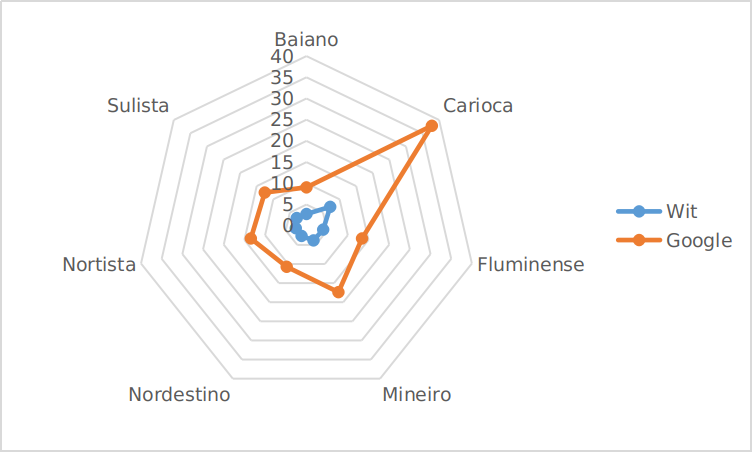
\includegraphics[width=.75\textwidth]{images/Lev_sotque_compont.png}
\fonte{elaborado pelo próprio autor (2021)}
\end{figure}

Analisando estes resultados, é possível se conjecturar que ambas as ferramentas não foram treinadas com o sotaque carioca e que este  sotaque tem características fonéticas bem diferentes, a tal ponto a prejudicar a transcrição da fala. 

\section{RESULTADO POR GÊNERO}

Nesta seção serão discutidos os resultados por gênero. O \autoref{Tabela_genero_Google_com_pontuacao} apresenta os resultados do Google Cloud considerando a pontuação para os diferentes gêneros e o \autoref{Tabela_genero_Google_sem_pontuacao} são os resultados sem considerar a pontuação. 
O \autoref{Tabela_genero_Wit_com_pontuacao} apresenta os resultados do Wit.ai considerando a pontuação para os diferentes gêneros e o \autoref{Tabela_genero_Wit_sem_pontuacao} são os resultados sem considerar a pontuação. 

Os resultados do Google Cloud são melhores para o gênero feminino que o do masculino. Nos resultados do  Wit.ai também, mas a diferença é bem pequena podendo ser considerada equiparável. 

%COM PONTUAÇÃO
\begin{quadro}[h]
\caption{Resultado do Google Cloud considerando a pontuação para análise entre gêneros} \label{Tabela_genero_Google_com_pontuacao}
\centering
\begin{tabular}{l|l|r|r|}
\hline
\multicolumn{1}{|c|}{Google Cloud}                            & Estatística   & \multicolumn{1}{l|}{Feminino} & \multicolumn{1}{l|}{Masculino} \\ \hline
\multicolumn{1}{|c|}{\multirow{2}{*}{Levenshtein}}            & Média         & \textbf{18,01}                       & 18,58                        \\ \cline{2-4} 
\multicolumn{1}{|c|}{}                                        & Mediana       & \textbf{13}                            & 15                             \\ \hline
\multicolumn{1}{|l|}{\multirow{2}{*}{\begin{tabular}[c]{@{}c@{}}Normalized \\ Levenshtein\end{tabular}}} & Média         & \textbf{89\%}                        & \textbf{89\%}                         \\ \cline{2-4} 
\multicolumn{1}{|l|}{}                                        & Mediana       & \textbf{92\%}                        & 91\%                         \\ \hline
\textbf{}                                                     & \# Acertos    & 0                             & 0                              \\ \cline{2-4} 
\textbf{}                                                     & \% de Acertos & 0\%                             & 0\%                              \\ \cline{2-4} 
\end{tabular}
\fonte{elaborado pelo próprio autor (2021)}
\end{quadro}

\begin{quadro}[h]
\caption{Resultado do Google Cloud sem considerar a pontuação para análise entre gêneros}
\label{Tabela_genero_Google_sem_pontuacao}
\centering
\begin{tabular}{l|l|r|r|}
\hline
\multicolumn{1}{|c|}{Google Cloud}                            & Estatística   & \multicolumn{1}{l|}{Feminino} & \multicolumn{1}{l|}{Masculino} \\ \hline
\multicolumn{1}{|c|}{\multirow{2}{*}{Levenshtein}}            & Média         & \textbf{13,26}                      & 13,85                       \\ \cline{2-4} 
\multicolumn{1}{|c|}{}                                        & Mediana       & \textbf{8}                             & 9                              \\ \hline
\multicolumn{1}{|l|}{\multirow{2}{*}{\begin{tabular}[c]{@{}c@{}}Normalized \\ Levenshtein\end{tabular}}} & Média         & \textbf{92\%}                      & 91\%                       \\ \cline{2-4} 
\multicolumn{1}{|l|}{}                                        & Mediana       & \textbf{95\%}                      & 94\%                        \\ \hline
\textbf{}                                                     & \# Acertos    & \textbf{80}                            & 46                             \\ \cline{2-4} 
\textbf{}                                                     & \% de Acertos & \textbf{9,36\%}                   & 5,80\%                     \\ \cline{2-4} 
\end{tabular}
\fonte{elaborado pelo próprio autor (2021)}
\end{quadro}





\begin{quadro}[h]
\caption{Resultado da Wit.ai  considerando a pontuação para análise entre gêneros} 
\label{Tabela_genero_Wit_com_pontuacao}
\centering
\begin{tabular}{l|l|r|r|}
\hline
\multicolumn{1}{|c|}{Wit.ai}                                  & Estatística   & \multicolumn{1}{l|}{Feminino} & \multicolumn{1}{l|}{Masculino} \\ \hline
\multicolumn{1}{|c|}{\multirow{2}{*}{Levenshtein}}            & Média         & \textbf{5,75}                        & 5,94                         \\ \cline{2-4} 
\multicolumn{1}{|c|}{}                                        & Mediana       & \textbf{4}                             & \textbf{4}                              \\ \hline
\multicolumn{1}{|l|}{\multirow{2}{*}{\begin{tabular}[c]{@{}c@{}}Normalized \\ Levenshtein\end{tabular}}} & Média         & \textbf{96\%}                        & \textbf{96\%}                         \\ \cline{2-4} 
\multicolumn{1}{|l|}{}                                        & Mediana       & \textbf{97\%}                        & \textbf{97\%}                         \\ \hline
\textbf{}                                                     & \# Acertos    & \textbf{51}                            & 30                             \\ \cline{2-4} 
\textbf{}                                                     & \% de Acertos & \textbf{5,97\%}                        & 3,77\%                         \\ \cline{2-4} 
\end{tabular}
\fonte{elaborado pelo próprio autor (2021) com os dados do Braccent.}
\end{quadro}

%SEM PONTUAÇÃO
\begin{quadro}[h]
\caption{Resultado da Wit.ai sem considerar a pontuação para análise entre gêneros} \label{Tabela_genero_Wit_sem_pontuacao}
\centering
\begin{tabular}{l|l|r|r|}
\hline
\multicolumn{1}{|c|}{Wit.ai}                                  & Estatística   & \multicolumn{1}{l|}{Feminino} & \multicolumn{1}{l|}{Masculino} \\ \hline
\multicolumn{1}{|c|}{\multirow{2}{*}{Levenshtein}}            & Média         & 3,22                        & \textbf{3,20}                         \\ \cline{2-4} 
\multicolumn{1}{|c|}{}                                        & Mediana       & \textbf{2}                             & \textbf{2}                              \\ \hline
\multicolumn{1}{|l|}{\multirow{2}{*}{\begin{tabular}[c]{@{}c@{}}Normalized \\ Levenshtein\end{tabular}}} & Média         & \textbf{98\%}                        & \textbf{98\%}                         \\ \cline{2-4} 
\multicolumn{1}{|l|}{}                                        & Mediana       & \textbf{98\%}                        & \textbf{98\%}                         \\ \hline
\textbf{}                                                     & \# Acertos    & \textbf{292}                           & 251                            \\ \cline{2-4} 
\textbf{}                                                     & \% de Acertos & \textbf{34,19\%}                       & 31,61\%                        \\ \cline{2-4} 
\end{tabular}
\fonte{elaborado pelo próprio autor (2021)}
\end{quadro}


\FloatBarrier

\section{RESULTADO POR GRAU DE ESCOLARIDADE}

%\todo[inline]{Thalles, ainda falta vc colocar uma tabela com o total por nível de escolaridade}

Nesta seção serão discutidos os resultados por nível de ensino. O \autoref{Tabela_ensino_Google_com_pontuacao} apresenta os resultados do Google Cloud considerando a pontuação para os diferentes níveis de ensino da pessoa e o \autoref{Tabela_Ensino_Google_sem_pontuacao} são os resultados sem considerar a pontuação. 
O \autoref{Tabela_Ensino_Wit_com_pontuacao} apresenta os resultados do Wit.ai considerando a pontuação para os diferentes níveis de ensino da pessoa  e o \autoref{Tabela_Ensino_Wit_sem_pontuacao} são os resultados sem considerar a pontuação. 



\begin{quadro}[h]
\caption{Resultado do Google Cloud  considerando a pontuação para análise entre graus de ensino (In = Incompleto, Com = Completo)}
\label{Tabela_ensino_Google_com_pontuacao}
\centering
\begin{tabular}{c|c|c|c|c|c|c|c|}
\hline
\multicolumn{1}{|c|}{\begin{tabular}[c]{@{}c@{}}Google\\ Cloud\end{tabular}}                             & Estatística  & \begin{tabular}[c]{@{}c@{}}Médio \\ In\end{tabular} & \begin{tabular}[c]{@{}c@{}}Médio \\ Com\end{tabular} & \begin{tabular}[c]{@{}c@{}}Superior \\ In\end{tabular} & \begin{tabular}[c]{@{}c@{}}Superior \\ Com\end{tabular} & Mestrado       & Doutorado \\ \hline
\multicolumn{1}{|c|}{\multirow{2}{*}{Levenshtein}}                                                       & Média        & 15,27                                               & 21,02                                                & 19,07                                                  & 18,9                                                    & \textbf{15,18} & 16,75     \\ \cline{2-8} 
\multicolumn{1}{|c|}{}                                                                                   & Mediana      & 14                                                  & 17                                                   & 15                                                     & 13                                                      & \textbf{12}    & 14        \\ \hline
\multicolumn{1}{|c|}{\multirow{2}{*}{\begin{tabular}[c]{@{}c@{}}Normalized \\ Levenshtein\end{tabular}}} & Média        & \textbf{0,91}                                       & 0,87                                                 & 0,89                                                   & 0,89                                                    & \textbf{0,91}  & 0,90      \\ \cline{2-8} 
\multicolumn{1}{|c|}{}                                                                                   & Mediana      & \textbf{0,92}                                       & 0,90                                                 & 0,90                                                   & \textbf{0,92}                                           & \textbf{0,92}  & 0,91      \\ \hline
\multicolumn{1}{l|}{}                                                                                    & \# Acertos   & 0                                                   & 0                                                    & 0                                                      & 0                                                       & 0              & 0         \\ \cline{2-8} 
\multicolumn{1}{l|}{}                                                                                    & \% de Acerto & 0                                                   & 0                                                    & 0                                                      & 0                                                       & 0              & 0         \\ \cline{2-8} 
\end{tabular}
\fonte{elaborado pelo próprio autor (2021).}
\end{quadro}

\begin{quadro}[h]
\caption{Resultado do Google Cloud sem  considerar a pontuação para análise entre graus de ensino (In = Incompleto, Com = Completo)} \label{Tabela_Ensino_Google_sem_pontuacao}
\centering
\begin{tabular}{c|c|c|c|c|c|c|c|}
\hline
\multicolumn{1}{|c|}{\begin{tabular}[c]{@{}c@{}}Google\\ Cloud\end{tabular}}                             & Estatística  & \begin{tabular}[c]{@{}c@{}}Médio \\ In\end{tabular} & \begin{tabular}[c]{@{}c@{}}Médio \\ Com\end{tabular} & \begin{tabular}[c]{@{}c@{}}Superior \\ In\end{tabular} & \begin{tabular}[c]{@{}c@{}}Superior \\ Com\end{tabular} & Mestrado      & Doutorado \\ \hline
\multicolumn{1}{|c|}{\multirow{2}{*}{Levenshtein}}                                                       & Média        & \textbf{9,86}                                       & 16,51                                                & 14,30                                                  & 14,26                                                   & 10,40         & 11,98     \\ \cline{2-8} 
\multicolumn{1}{|c|}{}                                                                                   & Mediana      & 8                                                   & 11                                                   & 10                                                     & 8                                                       & \textbf{7}    & 9         \\ \hline
\multicolumn{1}{|c|}{\multirow{2}{*}{\begin{tabular}[c]{@{}c@{}}Normalized \\ Levenshtein\end{tabular}}} & Média        & \textbf{0,94}                                       & 0,90                                                 & 0,91                                                   & 0,91                                                    & \textbf{0,94} & 0,93      \\ \cline{2-8} 
\multicolumn{1}{|c|}{}                                                                                   & Mediana      & \textbf{0,95}                                       & 0,93                                                 & 0,93                                                   & \textbf{0,95}                                           & \textbf{0,95} & 0,94      \\ \hline
\multicolumn{1}{l|}{}                                                                                    & \# Acertos   & 3                                                   & 7                                                    & 18                                                     & \textbf{65}                                             & 23            & 10        \\ \cline{2-8} 
\multicolumn{1}{l|}{}                                                                                    & \% de Acerto & 8,33                                                & 6,42                                                 & 4,60                                                   & 9,12                                                    & \textbf{9,46} & 6,36      \\ \cline{2-8} 
\end{tabular}
\fonte{elaborado pelo próprio autor (2021).}
\end{quadro}

\begin{quadro}[h]
\caption{Resultado da Wit.ai considerando a pontuação para análise entre graus de ensino (In = Incompleto, Com = Completo)} \label{Tabela_Ensino_Wit_com_pontuacao}
\centering
\begin{tabular}{c|c|c|c|c|c|c|c|}
\hline
\multicolumn{1}{|c|}{Wit.ai}                                                                            & Estatística  & \begin{tabular}[c]{@{}c@{}}Médio \\ In\end{tabular} & \begin{tabular}[c]{@{}c@{}}Médio \\ Com\end{tabular} & \begin{tabular}[c]{@{}c@{}}Superior \\ In\end{tabular} & \begin{tabular}[c]{@{}c@{}}Superior \\ Com\end{tabular} & Mestrado      & Doutorado     \\ \hline
\multicolumn{1}{|c|}{\multirow{2}{*}{Levenshtein}}                                                       & Média        & 5,13                                                        & 7,16                                                      & 7,16                                                           & 5,50                                                         & \textbf{4,72} & 5,14          \\ \cline{2-8} 
\multicolumn{1}{|c|}{}                                                                                   & Mediana      & 5                                                           & 5                                                         & 5                                                              & \textbf{4}                                                   & \textbf{4}    & \textbf{4}    \\ \hline
\multicolumn{1}{|c|}{\multirow{2}{*}{\begin{tabular}[c]{@{}c@{}}Normalized \\ Levenshtein\end{tabular}}} & Média        & \textbf{0,97}                                               & 0,95                                                      & 0,95                                                           & 0,96                                                         & \textbf{0,97} & \textbf{0,97} \\ \cline{2-8} 
\multicolumn{1}{|c|}{}                                                                                   & Mediana      & \textbf{0,97}                                               & \textbf{0,97}                                             & 0,96                                                           & \textbf{0,97}                                                & \textbf{0,97} & \textbf{0,97} \\ \hline
\multicolumn{1}{l|}{}                                                                                    & \# Acertos   & 1                                                           & 1                                                         & 12                                                             & \textbf{47}                                                  & 12            & 8             \\ \cline{2-8} 
\multicolumn{1}{l|}{}                                                                                    & \% de Acerto & 2,77                                                        & 0,91                                                      & 3,06                                                           & \textbf{6,60}                                                & 4,93          & 5,09          \\ \cline{2-8} 
\end{tabular}
\fonte{elaborado pelo próprio autor (2021).}
\end{quadro}


%SEM PONTUAÇÃO
\begin{quadro}[h]
\caption{Resultado da Wit.ai sem considerar a pontuação para análise entre graus de ensino (In = Incompleto, Com = Completo)} \label{Tabela_Ensino_Wit_sem_pontuacao}
\centering
\begin{tabular}{c|c|c|c|c|c|c|c|}
\hline
\multicolumn{1}{|c|}{Wit.ai}                                                                             & Estatística  & \begin{tabular}[c]{@{}c@{}}Médio \\ In\end{tabular} & \begin{tabular}[c]{@{}c@{}}Médio \\ Com\end{tabular} & \begin{tabular}[c]{@{}c@{}}Superior \\ In\end{tabular} & \begin{tabular}[c]{@{}c@{}}Superior \\ Com\end{tabular} & Mestrado       & Doutorado     \\ \hline
\multicolumn{1}{|c|}{\multirow{2}{*}{Levenshtein}}                                                       & Média        & \textbf{2,02}                                       & 4,55                                                 & 4,27                                                   & 3,023                                                   & 2,18           & 2,37          \\ \cline{2-8} 
\multicolumn{1}{|c|}{}                                                                                   & Mediana      & 2                                                   & 2                                                    & 2                                                      & 2                                                       & 2              & \textbf{1}    \\ \hline
\multicolumn{1}{|c|}{\multirow{2}{*}{\begin{tabular}[c]{@{}c@{}}Normalized \\ Levenshtein\end{tabular}}} & Média        & \textbf{0,98}                                       & 0,97                                                 & 0,97                                                   & \textbf{0,98}                                           & \textbf{0,98}  & \textbf{0,98} \\ \cline{2-8} 
\multicolumn{1}{|c|}{}                                                                                   & Mediana      & \textbf{0,99}                                       & 0,98                                                 & 0,98                                                   & 0,98                                                    & \textbf{0,99}  & \textbf{0,99} \\ \hline
\multicolumn{1}{l|}{}                                                                                    & \# Acertos   & 9                                                   & 26                                                   & 115                                                    & \textbf{242}                                            & 95             & 56            \\ \cline{2-8} 
\multicolumn{1}{l|}{}                                                                                    & \% de Acerto & 25                                                  & 23,85                                                & 29,41                                                  & 33,98                                                   & \textbf{39,09} & 35,66         \\ \cline{2-8} 
\end{tabular}
\fonte{elaborado pelo próprio autor (2021).}
\end{quadro}
\FloatBarrier

\begin{figure}[h!]
\centering
\caption{Gráfico em rede comparando os resultados de Levenshtein, sem considerar a pontuação, do Wit.ai e do Google Cloud, por grau de escolaridade.}
\label{fig:rede2}
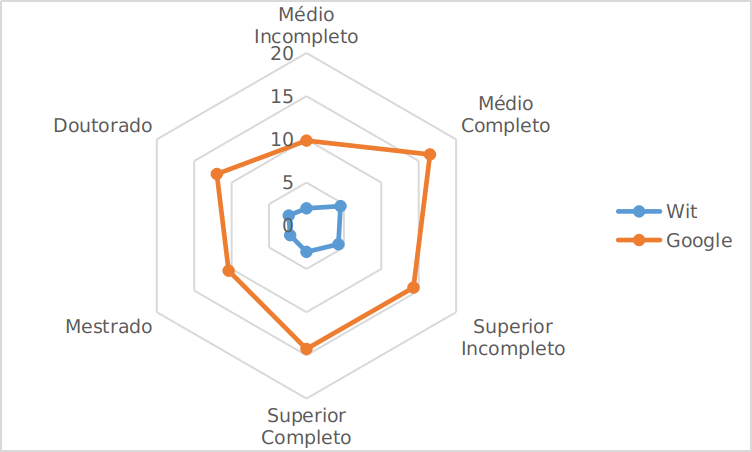
\includegraphics[width=.75\textwidth]{images/Lev_grau_sempont.png}
\fonte{elaborado pelo próprio autor (2021)}
\end{figure}

A \autoref{fig:rede2} apresenta um gráfico em rede comparando os resultados de Levenshtein, sem considerar a pontuação, em que cada ponta é um grau de escolaridade, a curva azul é o resultado do Wit.ai e a curva laranja é do Google Cloud. É possível notar que a curva de menor área é do Wit.ai, representando o melhor resultado em todos os graus de escolaridade. 
Pelos resultados, é possível verificar que o nível de ensino não é um fator discriminador para as ferramentas de transcrição considerando a base de dados usada. Se o nível de ensino fosse o fator discriminante, os valores das métricas melhorariam de acordo com o aumento do nível de ensino, e não é o que os resultados apresentam. 
%COM PONTUAÇÃO


